\documentclass[letterpaper]{l3doc}

\hypersetup{urlcolor = teal, filecolor = violet}
\usepackage[mono = false]{libertine}
\usepackage{pdfpages,hologo,framed}
\hologoFontSetup{general = \sffamily}
\FrameSep = 0pt
\usepackage[fontset = none]{ctex}
\setCJKmainfont[BoldFont = *-Bold]{LXGW WenKai}
\setCJKsansfont[BoldFont = *-Bold]{LXGW WenKai}
\setCJKmonofont[BoldFont = *-Bold]{LXGW WenKai}
\usepackage[os = mac]{menukeys}
\AddToHook{env/function/before}{\vspace*{-.5\baselineskip}}

\title
{
  \bfseries\cls{litetable} 文档类:多彩的课程表
  \thanks{\url{https://github.com/xiamyphys/litetable}}
}
\author
{
  夏明宇 \texttt{<\href{mailto:xiamyphys@gmail.com}{xiamyphys@gmail.com}>}
  \thanks{\href{https://github.com/ljguo1020}{郭李军}开发了读取 \meta{left} -> \meta{right} 型数据结构模块和低版本 \hologo{TeX} Live 兼容模块.}
}
\date{Version 3.1A, \today}

\begin{document}

\maketitle

\section{介绍}

\cls{litetable} 文档类提供了一个多彩的课程表设计,基于 \cls{article} 文档类,由 \pkg{expl3} 和 \pkg{tikz} 构建. 兼容发行版 \hologo{TeX} Live 2021及更高版本,在 \hologo{pdfLaTeX} 和 \hologo{XeLaTeX} 编译器下均可正常运行. 本文档为 \cls{litetable} 文档类的中文用户手册,手册同时有\href{./litetable-en.pdf}{英文}和\href{./litetable-hk.pdf}{粤语}版本\footnote{\href{https://qm.qq.com/q/RyssAhG4qy}{QQ Group: 760570712}}.

\section{载入 \cls{litetable} 并生成课程表框架}

同加载其他文档类一样,只需写下

\begin{framed}
  \begin{verbatim}
    \documentclass{litetable}
  \end{verbatim}
\end{framed}

如果用户需要输入中文,可自行载入 \pkg{ctex} 宏包并设置字体.

\begin{function}{\timelist,\weeklist}
  \begin{syntax}
    \cs{timelist}\oarg{rows}\marg{time list}             \cs{timelist}\marg{time list}\oarg{rows}
    \cs{weeklist}\oarg{default weeks}\marg{week list}    \cs{weeklist}\marg{week list}\oarg{default weeks}
  \end{syntax}

  以上命令均有两个参数. 命令 \cs{timelist} 的可选参数可直接决定课程表的行数,命令 \cs{weeklist} 的可选参数可决定默认的星期数目并会在每个课程块的右下角显示. 两个命令的强制参数均接收数组,可分别在课程表的左侧添加时间列表、在课程表的顶部添加对应宽度比例的工作日.

  若命令 \cs{timelist} 中时间数组数目大于可选参数接收值,则多余的时间数组将被忽略,并返回一个警告. 如果只在课程表左侧添加一列序号,使强制参数为空即可.
\end{function}

\begin{function}{\more}
  \begin{syntax}
    \cs{more}\marg{comment}
  \end{syntax}

  此命令可在页面的右下角添加备注.
\end{function}

\begin{function}{\maketable}
  \begin{syntax}
    \cs{maketable}\oarg{semester}\marg{title}            \cs{maketable}\marg{title}\oarg{semester}
  \end{syntax}

  此命令有两个参数,可生成一个空白的课程表框架,需在命令 \cs{timelist},\cs{weeklist} 和 \cs{more} 后,并在带有 \cmd{[remember picture, overaly]} 选项的 \env{tikz} 环境中执行. 可选参数可在页面的右上角添加学期块,强制参数可指定标题.
\end{function}

\section{添加课程块}

\begin{function}{\course}
  \begin{syntax}
    \cs{course}\oarg{keyvals}\marg{start number}\marg{end number}
  \end{syntax}

  \cs{course} 命令可在当前工作日添加课程块,需在命令 \cs{maketable} 后,并在带有 \cmd{[remember picture, overaly]} 选项的 \env{tikz} 环境中执行.
  
  此命令有三个参数. 第一个可选参数接收下列键:\keys{\cmdmac~color} \keys{\cmdmac~subject} \keys{\cmdmac~location} \keys{\cmdmac~teacher} \keys{\cmdmac~weeks}. 键 \keys{\cmdmac~color} 默认值为 \cmd{teal},键 \keys{\cmdmac~weeks} 默认值由命令 \cs{weeklist} 的可选参数决定. 第二个和第三个强制参数分别为课程的开始和结束序号.

  \cs{course} 命令的用例如下:将此课程块的颜色设置为 \cmd{DarkSlateGray},此课程名称为 \cmd{litetable},上课地点为 \cmd{Hong Kong},教师为 \cmd{M.Y. Xia},在当日的第 \cmd{8} 节课开始,第 \cmd{8} 节课结束.
  
  \begin{framed}
    \begin{verbatim}
    \course [ color = DarkSlateGray, subject = litetable,
              location = Hong Kong, teacher = M.Y. Xia
            ] {8} {8}
    \end{verbatim}
  \end{framed}
  
  \begin{itemize}[topsep = 0pt]
    \item 若课程块的高度只有一格,即$\meta{start number} = \meta{end number}$,则键 \keys{\cmdmac~location} 和 \keys{\cmdmac~teacher} 的值将输出在同一行并以逗号 (,) 间隔,键 \keys{\cmdmac~weeks} 的值将会隐藏.
    \item 若键 \keys{\cmdmac~location} 和 \keys{\cmdmac~teacher} 均未赋值,则键 \keys{\cmdmac~subject} 的值将输出在课程块中心.
    \item 超出课程表工作日范围的课程块将不会显示,只会返回一条警告.
  \end{itemize}
\end{function}

\begin{function}{\newday}
  \begin{syntax}
    \cs{newday}\oarg{integral value}
  \end{syntax}

  此命令有一个可选参数,可使其后面添加的课程块后移 \meta{intergal value} 个工作日. 可选参数的默认值为 \cmd{1},即后移 \cmd{1} 个工作日.
\end{function}

\clearpage

\section{最小工作示例}

此MWE生成的课程表有13行但是只有前12行标注时间,课程表顶部共有5个工作日,工作日之间的宽度比例为$4:5:4:6:5$,键 \keys{\cmdmac~weeks} 的默认值被赋为 \cmd{Weeks 1 - 16}. 添加了注释和两个课程块.

\begin{framed}
  \begin{verbatim}
    \documentclass{litetable}

    \begin{document}

    \timelist[13]
    {
      08:05 -> 08:50, 08:55 -> 09:40, 10:00 -> 10:45, 10:50 -> 11:35,
      11:40 -> 12:25, 13:30 -> 14:15, 14:20 -> 15:05, 15:15 -> 16:00,
      16:05 -> 16:50, 18:30 -> 19:15, 19:20 -> 20:05, 20:10 -> 20:55
    }
    \weeklist[Weeks 1 - 16]
    {
      Mon -> 4, Tue -> 5, Wed -> 4, Thu -> 6, Fri -> 5
    }
    \more{Author: Mingyu Xia \& Lijun Guo}

    \begin{tikzpicture}[remember picture, overlay]
      \maketable
      \course [ subject = Keep on {\TeX}ing
              ] {10} {11}
      \newday
      \course [ color = DarkSlateGray, subject = litetable,
              location = Hong Kong, teacher = M.Y. Xia
              ] {8} {8}
    \end{tikzpicture}

    \end{document}
  \end{verbatim}
\end{framed}

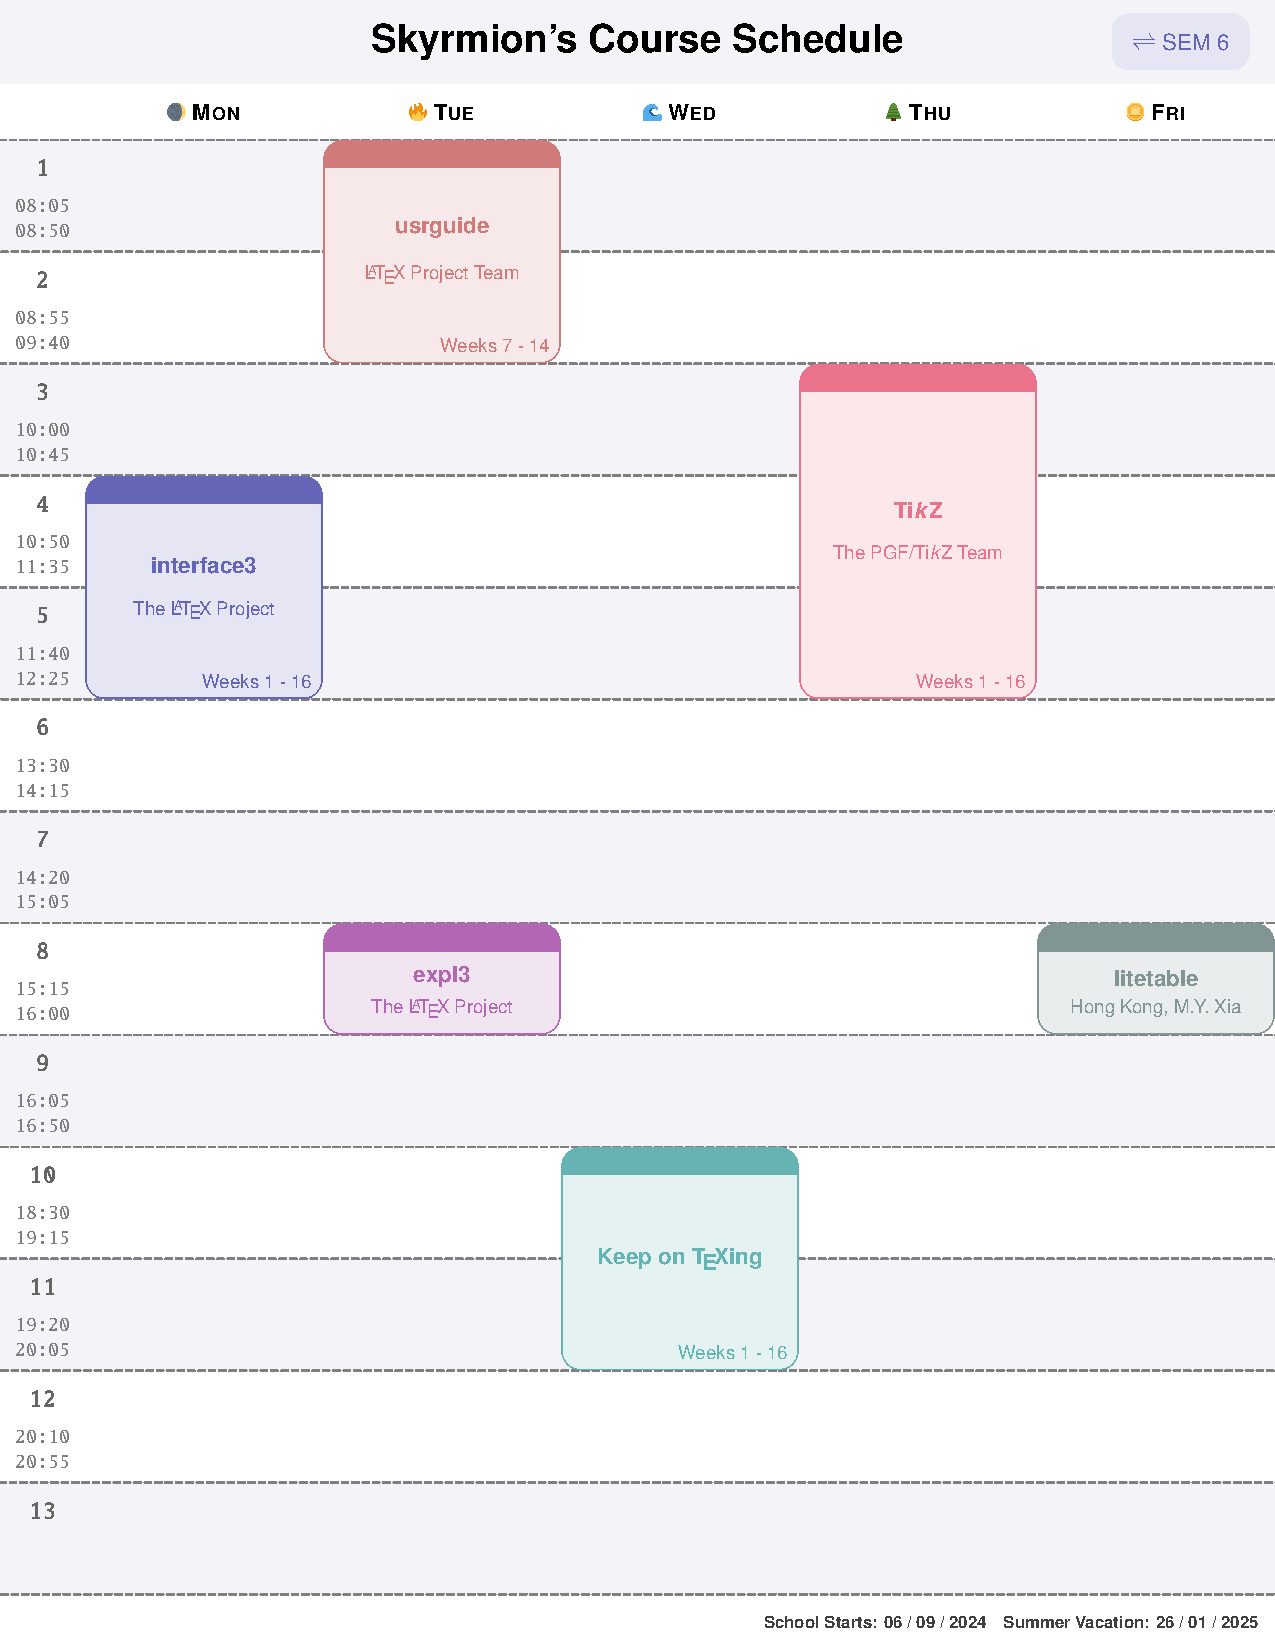
\includepdf[pages = 1]{litetable-demo.pdf}

\end{document}